\chapter{CUDA}

CUDA\cite{hendarto2017performance} (acronimo di Compute Unified Device Architecture) è un'architettura hardware per l'elaborazione parallela creata da NVIDIA. Tramite l'ambiente di sviluppo per CUDA, i programmatori di software possono scrivere applicazioni capaci di eseguire calcolo parallelo sulle GPU delle schede video NVIDIA.

CUDA dà accesso agli sviluppatori ad un set di istruzioni native per il calcolo parallelo di elementi delle GPU CUDA. Usando CUDA, le ultime GPU Nvidia diventano in effetti architetture aperte come le CPU. Diversamente dalle CPU, le GPU hanno un'architettura parallela con diversi core, ognuno capace di eseguire centinaia di processi simultaneamente: se un'applicazione è adatta per questo tipo di architettura, la GPU può offrire grandi prestazioni e benefici.

Dato l'aumentare della complessità dei algoritmi di criptazione nel tempo, questo tipo di tecnologia è diventata molto popolare nell'esecuzione del Brute Force. 

\section{CPU vs GPU}

Diversi tool per il Brute Force ormai permettono l'utilizzo delle GPU insieme alle CPU per eseguire le computazioni per estrarre le password dagli hash. Uno di questi strumenti è Hashcat.

\begin{figure}[ht]
    \centering
    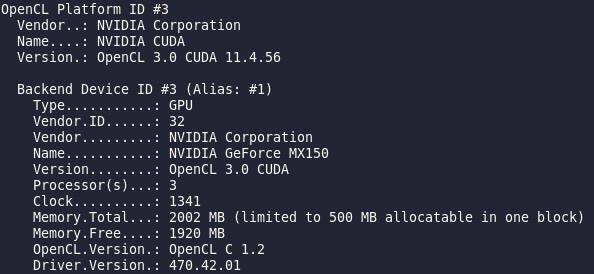
\includegraphics[width=\linewidth]{Immagini/7/GPU_hashcat.png}
    \caption{GPU hashcat}
\end{figure}

\newpage

L'utilizzo della forza computazionale delle GPU, come detto, risulta molto più efficente delle CPU, ecco riportati dei esempi delle differenze delle velocità di calcolo su diversi tipi di algoritmi di criptazione.
\newline

\#1 -> NVIDIA GeForce MX150 - 2048 MB, Core: 1341 MHz, Memoria: 1253 MHz, GDDR5, 382.64, Optimus

\#2 -> Intel Corporation UHD Graphics 620 1.150 MHz

\#3 -> Intel Core i7-8550U CPU @ 1.80GHz

\begin{figure}[ht]
    \centering
    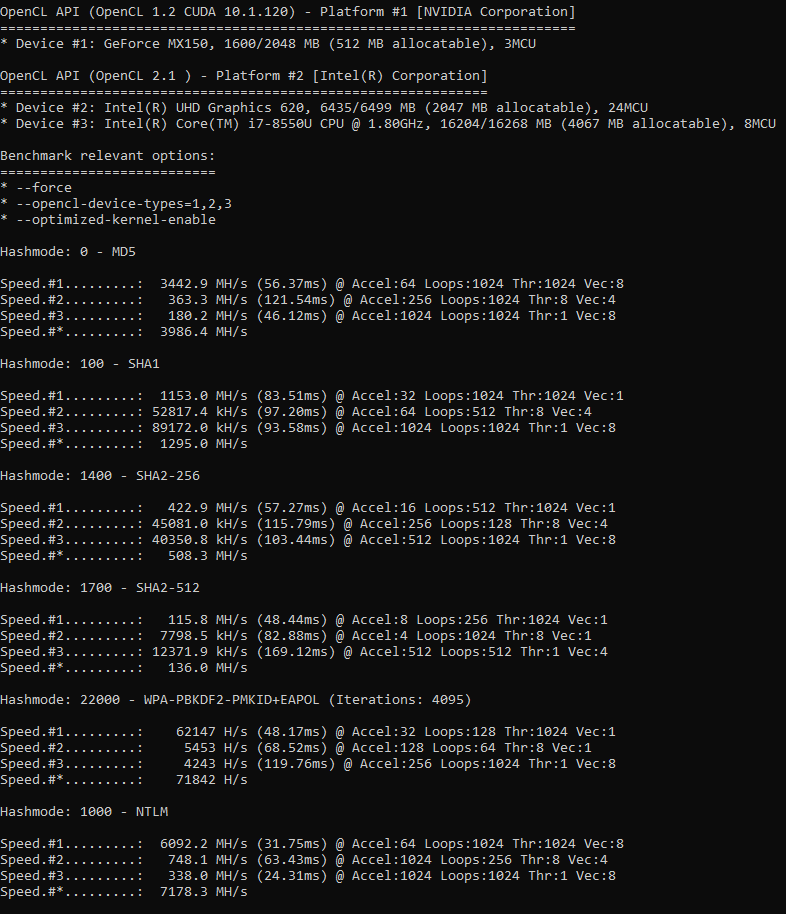
\includegraphics[width=\linewidth]{Immagini/7/cpu_gpu.PNG}
    \caption{CPU vs GPU}
    \label{fig:CPU vs GPU}
\end{figure}

\label{chap:conc}